\documentclass[tikz,border=8pt]{standalone}
\usepackage{amsmath}
\usetikzlibrary{arrows.meta,decorations.pathreplacing}
\begin{document}

% Asset ID: AS2DataPresentationTikZ-001
% Source: Box plot recap evidence.
% Related lesson section: Core Theory, Box Plots.
% Purpose: Label minimum, Q_1, median, Q_3, maximum, IQR and range.
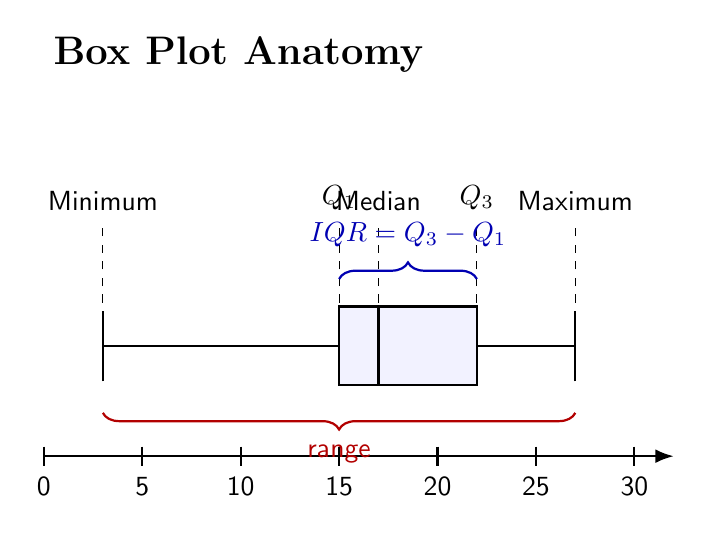
\begin{tikzpicture}[x=0.25cm,y=1cm,>=Latex,font=\sffamily]
\node[anchor=west,font=\bfseries\Large] at (0,5.1) {Box Plot Anatomy};
\draw[->,thick] (0,0) -- (32,0);
\foreach \x in {0,5,10,15,20,25,30}{\draw[thick] (\x,0.12)--(\x,-0.12);\node[below] at (\x,-0.15){\x};}
\draw[thick] (3,1.4)--(15,1.4); \draw[thick] (22,1.4)--(27,1.4);
\draw[thick,fill=blue!5] (15,0.9) rectangle (22,1.9); \draw[thick] (17,0.9)--(17,1.9);
\draw[thick] (3,0.95)--(3,1.85); \draw[thick] (27,0.95)--(27,1.85);
\foreach \x/\t in {3/Minimum,15/$Q_1$,17/Median,22/$Q_3$,27/Maximum}{\draw[dashed] (\x,1.95)--(\x,3);\node[above,align=center] at (\x,3){\t};}
\draw[decorate,decoration={brace,amplitude=6pt},thick,blue!70!black] (15,2.25)--(22,2.25) node[midway,above=8pt] {$IQR=Q_3-Q_1$};
\draw[decorate,decoration={brace,amplitude=6pt,mirror},thick,red!70!black] (3,0.55)--(27,0.55) node[midway,below=8pt] {range};
\end{tikzpicture}

\end{document}
